% ===========================================================================
% SECTION 4  MACHINE LEARNING SURROGATE MODELS
% Target: 1500-2000 words
% ===========================================================================

\section{Machine Learning Surrogate Models}
\label{sec:ml_surrogates}

All surrogates are trained on the Stage~1 dataset
(Section~\ref{sec:dataset_generation}) to predict the one-step-ahead state
$[\omegar^{+},\beta^{+}]$ from $X=[\omegar,\beta,V,u_{\text{cmd}}]$, using the
shared global normalization computed on the training split. Two naive
baselines are reported for reference: \emph{Persistence}
($\hat{x}^{+}=x$) and a \emph{Linear ARX} model fitted by ordinary least
squares. All six surrogate architectures below are trained and evaluated
under the same protocol.

\subsection{V1 Models}
\label{subsec:v1_models}

\subsubsection{Local Linear Neuro-Fuzzy Model (LLNFM / ANFIS)}
\label{subsubsec:llnfm}

The LLNFM surrogate is implemented as two independent Sugeno-type
ANFIS \citep{jang_anfis_1993} networks (one per output channel), each
with a grid-partitioned rule base
of $2$ generalized bell membership functions (\texttt{gbellmf}) per input,
giving $2^4=16$ fuzzy rules, $55$ network nodes, and $104$ total parameters
($80$ linear consequent parameters, $24$ nonlinear premise parameters).
Training uses MATLAB's \texttt{anfis()} function on a $3{,}000$-point
subsample of the training set for $80$ epochs. We note that the
\texttt{tunefis()} API (the object-oriented ANFIS training interface
introduced in recent MATLAB releases) proved incompatible in R2024a and
could not be used; the legacy matrix-based \texttt{anfis()} syntax was
confirmed to work correctly and was used throughout this study. The omega
sub-network converges quickly (error goal reached at epoch~2), while the
beta sub-network trains for the full $80$ epochs without reaching the error
goal, oscillating around a training RMSE of $\approx 0.013$--$0.017$ in
normalized units. Despite this, LLNFM achieves the best test-set accuracy
among all V1 surrogates: $\RMSE_{\omega} = \SI{0.0088}{rpm}$,
$\RMSE_{\beta} = 0.0964\deg$, in $\SI{8.2}{s}$ of training time.

\subsubsection{Gaussian Process (V1)}
\label{subsubsec:gp_v1}

The V1 Gaussian Process surrogate uses a Squared-Exponential (SE) kernel
with default (non-optimized) hyperparameters, fitted independently for each
output on a $N_{\text{sub}}=400$-point subsample (to keep the $O(N^3)$
training cost tractable). Training completes in $\SI{4.0}{s}$, and the
model achieves $\RMSE_{\omega} = \SI{0.0066}{rpm}$, $\RMSE_{\beta} =
0.1427\deg$ on the test set  matching LLNFM as the best-performing V1
surrogate on rotor speed. The mean predictive standard deviation on the
test set, $\sigma_{\text{te}} = [0.00108,\ 0.15139]$ (omega, beta, raw
units), is retained for comparison against the calibrated V2 uncertainty
(Section~\ref{subsubsec:gp_v2}).

\subsubsection{Physics-Informed Neural Network (V1)}
\label{subsubsec:pinn_v1}

The PINN surrogate is a fully-connected MLP with hidden layers of size
$64$--$64$--$32$, trained for $3{,}000$ iterations with mini-batch size
$256$ and a step-decayed learning rate (initial $10^{-3}$, halved every
$400$ iterations). The loss combines a data term with a physics residual
term derived from the rotor ODE (Eq.~\eqref{eq:rotor_ode}), weighted by
$\lambda_{\text{phy}} = 0.10$. A physics residual on the pitch channel was
deliberately excluded: since the simulation time step equals the pitch
actuator time constant ($\Delta t = \tau_\beta = \SI{0.1}{s}$), the exact
discrete pitch-actuator ODE degenerates to $\beta^{+} = u_{\text{cmd}}$,
which conflicts with the pitch-rate saturation present in the real
(simulated) data; including this residual was found to actively hurt
training. Training converges to a total loss of $\approx 0.0008$ by
iteration $3{,}000$ ($\SI{114.5}{s}$ total training time), yielding
$\RMSE_{\omega} = \SI{0.0183}{rpm}$, $\RMSE_{\beta} = 0.1924\deg$  a
$3.1\%$ \emph{degradation} relative to the Linear ARX baseline, the only V1
surrogate to underperform the linear reference.

\subsubsection{Long Short-Term Memory (V1)}
\label{subsubsec:lstm_v1}

The LSTM \citep{hochreiter_lstm_1997} surrogate uses a sequence length of $10$ steps and two stacked
LSTM layers ($64$ and $32$ units) with $10\%$ dropout, trained for $60$
epochs (Adam, learning rate $10^{-3}$, batch size $64$) on trajectory-
respecting sequences ($16{,}240$ train / $3{,}480$ validation / $3{,}480$
test sequences, consistent with the trajectory-based split of
Section~\ref{subsec:dataset_structure}). Training required $\SI{2136.1}{s}$
($\approx\SI{36}{min}$)  three orders of magnitude slower than the other
V1 surrogates  and achieved $\RMSE_{\omega}=\SI{0.0147}{rpm}$,
$\RMSE_{\beta}=0.2083\deg$, a modest $+17.1\%$ gain over the linear
baseline but markedly worse than LLNFM or GP. As shown in
Section~\ref{subsec:operational_feasibility}, this accuracy is in any case
moot: LSTM inference cost renders the model unusable inside the closed-loop
MPC. We attribute the limited benefit of the recurrent architecture to the
system's own dynamics: because $\Delta t = \tau_\beta$, the informative
history genuinely required for one-step prediction is short, so a
$10$-step memory window offers little advantage over the instantaneous
state  a hypothesis further supported by the V2 TCN/SW-MLP results
(Section~\ref{subsubsec:tcn_swmlp}).

\subsection{V2 Improvements}
\label{subsec:v2_models}

The V1 dataset (Section~\ref{sec:dataset_generation}) is reused unchanged
for V2 training. LLNFM is carried over from V1 without modification. Two
new sequence-based architectures (TCN, SW-MLP) are introduced to test the
memory-window hypothesis raised in Section~\ref{subsubsec:lstm_v1}, and the
GP and PINN surrogates are upgraded as described below.

\subsubsection{GP-v2 (Matérn 5/2 + Optimized Hyperparameters)}
\label{subsubsec:gp_v2}

Two changes are introduced relative to the V1 GP. First, the kernel is
changed from Squared-Exponential to Matérn~5/2,
$k(r) = \left(1 + \tfrac{\sqrt{5}r}{l} + \tfrac{5r^2}{3l^2}\right)
\exp\!\left(-\tfrac{\sqrt{5}r}{l}\right)$, which assumes only twice
differentiable sample paths rather than infinite smoothness  a weaker and
more physically appropriate regularity assumption for a system subject to
turbulent forcing \citep{rasmussen2006}. Second, hyperparameters
$(\sigma_f, l, \sigma_n)$ are tuned by Bayesian optimization (marginal
likelihood objective, $20$ evaluations) rather than left at default values.
An earlier training pass inadvertently let this same Bayesian search
also select the kernel family itself, silently overriding the intended
Mat\'ern~5/2 choice with an ARD-Exponential kernel; this has been
fixed by restricting the optimized hyperparameter set to length scale
and noise variance only. \textbf{Verification}: loading the trained
model and inspecting its \texttt{KernelFunction} property directly
confirms \texttt{Matern52} for both output channels of GP-v2, distinct
from V1's confirmed \texttt{SquaredExponential}, with
\texttt{isequal} false between the two model objects -- ruling out a
stale-workspace or copy-paste explanation for any subsequent numerical
similarity between V1 and V2 results. The optimized hyperparameters
(length scale $l$, signal deviation $\sigma_f$, noise deviation
$\sigma_n$) differ substantially between the two output channels: for
$\omegar^{+}$, $l=109.35$, $\sigma_f=3.152$, $\sigma_n=0.0052$; for
$\beta^{+}$, $l=996.68$, $\sigma_f=5281.3$, $\sigma_n=0.0729$ -- the
large length scale on the beta channel reflecting the near-linear,
low-curvature relationship between normalized
inputs and $\beta^{+}$. Training takes $\SI{50.4}{s}$ (versus
$\SI{4.5}{s}$ for V1, a one-time cost with no impact on inference), and
test accuracy reaches $\RMSE_{\omega}=\SI{0.0129}{rpm}$,
$\RMSE_{\beta}=0.1448\deg$ -- a $26.3\%$ gain over the linear baseline
on the $\omega$ channel, though worse than both V1 GP
($\SI{0.0083}{rpm}$) and V1 LLNFM ($\SI{0.0088}{rpm}$) in absolute
terms, and not the best $\beta$ accuracy of any surrogate evaluated
either (LLNFM's $\SI{0.0964}{deg}$ remains lower). GP-v2 is not the
best-accuracy surrogate on either channel; its practical advantage,
discussed next, is calibrated predictive uncertainty rather than
raw accuracy. Critically,
the Bayesian-optimized hyperparameters directly calibrate the predictive
uncertainty $\sigma_{\text{te}}$, which motivates the GP-based
uncertainty-penalized MPC cost introduced in
Section~\ref{subsec:gp_uncertainty_cost}.

\subsubsection{PINN-v2 (Differentiable Softplus)}
\label{subsubsec:pinn_v2}

The V1 PINN clips the power coefficient with
$C_{p}^{\text{clip}} = \max(0,\ \min(C_{p,\text{Betz}},\ C_{p}))$ to enforce
physical bounds in the residual term, which is non-differentiable at the
clipping boundaries and produces a zero gradient exactly where the physics
loss is most active. In PINN-v2, this is replaced with a smooth softplus
saturation, keeping the physics residual differentiable everywhere in the
training domain. Training settings are otherwise unchanged ($3{,}000$
iterations, $\lambda_{\text{phy}}=0.10$). Test accuracy improves modestly relative to V1
($\RMSE_{\omega}=\SI{0.0193}{rpm}$ vs.\ $\SI{0.0183}{rpm}$,
$\Delta=\SI{0.0010}{rpm}$, $\approx5.2\%$ relative -- since PINN-v2's
training seed is now explicitly recorded (Appendix~\ref{subsec:appendix_seeding})
but V1's original run predates that fix, we cannot rule out
run-to-run initialization variance as a contributor to this small
difference, rather than the architectural change alone);
$\RMSE_{\beta}=0.1636\deg$ vs.\ $0.1924\deg$), and PINN-v2 remains, along
with TCN, one of the two surrogates that fail to outperform the linear
baseline ($-4.5\%$). The differentiable formulation therefore did not
translate into a measurable accuracy gain on this dataset, though it
removes a documented source of ill-conditioned gradients during training.

\subsubsection{TCN and SW-MLP (New Architectures)}
\label{subsubsec:tcn_swmlp}

Two new sequence-based surrogates are introduced specifically to test
whether the poor cost-effectiveness of LSTM (Section~\ref{subsubsec:lstm_v1})
is a limitation of the recurrent architecture itself or a more fundamental
consequence of the system's short effective memory. The \emph{Temporal
Convolutional Network} (TCN) uses a $10$-step input window with dilated
causal 1-D convolutions (dilations $1,2,4$), $16$ filters, kernel size
$3$, and global average pooling ($1{,}906$ parameters total), trained for
$60$ epochs. The \emph{Sliding-Window MLP} (SW-MLP) instead flattens the
same $10$-step window into a single $40$-dimensional input vector
(\texttt{featureInputLayer}) fed to a $64$--$32$ MLP ($4{,}770$
parameters), trained under the same protocol. Results are markedly
different: TCN performs \emph{worse} than persistence
($\RMSE_{\omega}=\SI{0.0469}{rpm}$, $-154.1\%$ vs.\ linear), while SW-MLP
achieves a modest positive gain ($\RMSE_{\omega}=\SI{0.0171}{rpm}$,
$+7.5\%$). Neither architecture approaches the accuracy of the
instantaneous-state surrogates (LLNFM, GP-v2). This result reinforces the
hypothesis raised in Section~\ref{subsubsec:lstm_v1}: because
$\Delta t = \tau_\beta$, the $10$-step temporal window is largely redundant
information for one-step prediction, and windowed/recurrent architectures
pay a real optimization and capacity cost for modeling a temporal
dependency the plant does not strongly exhibit at this sampling rate. TCN's
particularly poor result  worse than naive persistence  suggests the
causal-dilated convolutional inductive bias is actively mismatched to this
near-memoryless dynamics, though we do not rule out that further
hyperparameter tuning could narrow this gap; this is noted as a limitation
in Section~\ref{subsec:limitations}.

\subsection{Comparative Prediction Accuracy}
\label{subsec:comparative_accuracy}

Table~\ref{tab:stage2_accuracy} summarizes test-set accuracy for all
V1 and V2 surrogates. LLNFM (V1, unchanged in V2) achieves the best
pitch-channel accuracy overall ($\RMSE_{\beta}=0.0964\deg$); GP-v2 is
close but not best on this channel ($\RMSE_{\beta}=0.1448\deg$,
comparable to V1 GP's $0.1437\deg$). On the rotor-speed channel, GP-v2's
$\RMSE_{\omega}=\SI{0.0129}{rpm}$ is higher (worse) than V1 GP
($\SI{0.0083}{rpm}$) and both LLNFM figures ($\SI{0.0088}{rpm}$);
within the V2 snapshot alone, GP-v2 no longer edges out
LLNFM$^{*}$ on $\omega$ either. LLNFM remains the best
accuracy-per-training-second trade-off ($\SI{8.2}{s}$ vs.\
$\SI{50.4}{s}$ for GP-v2). Against the Linear ARX baseline, LSTM, TCN,
and V1 PINN fail to clearly outperform it, while V2's PINN-v2 now
edges narrowly ahead ($+1.6\%$); TCN performs worse than even the
naive Persistence baseline on this dataset.

We note one clarification for rigor, updated from an earlier draft of
this paper. A previous version of the pipeline generated V2's dataset
via a separate, deliberately widened generator (covering Region~II
explicitly, alongside the V1-style near-rated initialization), so that
V1 and V2 were evaluated on genuinely different test-set
distributions and were reported as non-comparable snapshots for that
reason. Following the physical-parameter correction of
Section~\ref{subsec:torque_switching}, the pipeline was consolidated
to a single, unified \texttt{stage1\_generate\_data.m} used by both V1
and V2 training runs; the separate V2-specific generator no longer
exists. Persistence and LLNFM (both unretrained-or-parameter-free
components) accordingly now report numerically identical figures in
both snapshots (Table~\ref{tab:stage2_accuracy}), which is the
expected, correct behavior for models evaluated on the same test set
-- not a discrepancy requiring explanation. V1 and V2 are still
reported as two snapshots because they reflect two distinct sets of
trained \emph{surrogate architectures} (V1: LLNFM, LSTM, GP, PINN; V2
adds/replaces with TCN, SW-MLP, GP-v2, PINN-v2), not because of any
remaining difference in the underlying data. Gains relative to Linear
ARX (Table~\ref{tab:stage2_accuracy}, last column) are computed
against a single shared Linear ARX baseline for this reason. All
figures in Table~\ref{tab:stage2_accuracy} were regenerated with an
explicit, recorded random seed (\texttt{cfg.data.split\_seed}) fixed
before every stochastic training step, confirmed reproducible across
repeated runs on the same MATLAB release.

\begin{table}[H]
\centering
\caption{Comparative one-step prediction accuracy of all surrogates,
V1 and V2 snapshots (test set, $N=3{,}600$ samples). V2 figures use
explicit, recorded random seeds (Appendix~\ref{sec:appendix}) and are
confirmed reproducible.}
\label{tab:stage2_accuracy}
\begin{tabular}{llcccc}
\toprule
Snapshot & Model & RMSE-$\omega$ (rpm) & RMSE-$\beta$ (deg) & Train (s) & Gain vs.\ Linear \\
\midrule
\multirow{6}{*}{V1}
 & Persistence  & 0.0241 & 0.3220 & --    & $-38.1\%$ \\
 & Linear ARX   & 0.0175 & 0.1420 & $<1$  & reference \\
 & LLNFM        & 0.0088 & 0.0964 & 8.2   & $+49.5\%$ \\
 & LSTM         & 0.0207 & 0.2056 & 685.8 & $-18.3\%$ \\
 & GP           & 0.0083 & 0.1437 & 4.5   & $+52.6\%$ \\
 & PINN         & 0.0178 & 0.1738 & 61.4  & $-2.0\%$ \\
\midrule
\multirow{7}{*}{V2}
 & Persistence  & 0.0241 & 0.3220 & --    & $-38.1\%$ \\
 & Linear ARX   & 0.0175 & 0.1420 & $<1$  & reference \\
 & LLNFM$^{*}$  & 0.0088 & 0.0964 & 8.2   & $+49.5\%$ \\
 & TCN          & 0.0396 & 0.3511 & 1248.3 & $-126.9\%$ \\
 & SW-MLP       & 0.0154 & 0.1612 & 193.6 & $+12.1\%$ \\
 & GP-v2        & 0.0129 & 0.1448 & 50.4  & $+26.3\%$ \\
 & PINN-v2      & 0.0172 & 0.1738 & 57.8  & $+1.6\%$ \\
\bottomrule
\end{tabular}

\vspace{4pt}
{\footnotesize $^{*}$LLNFM architecture and weights unchanged from V1.
V1 and V2 now share a single, unified Stage~1 dataset (regenerated
after the physical-parameter correction of
Section~\ref{subsec:torque_switching}); consequently LLNFM's V1 and V2
figures are numerically identical, as expected for an unretrained
model evaluated on the same test set. An earlier draft of this table
reported a V1/V2 discrepancy for LLNFM, attributed at the time to a
deliberately widened V2-specific test set; that separate V2 dataset
generator no longer exists in the current, consolidated pipeline, and
the discrepancy no longer arises.}
\end{table}

\begin{figure}[H]
\centering
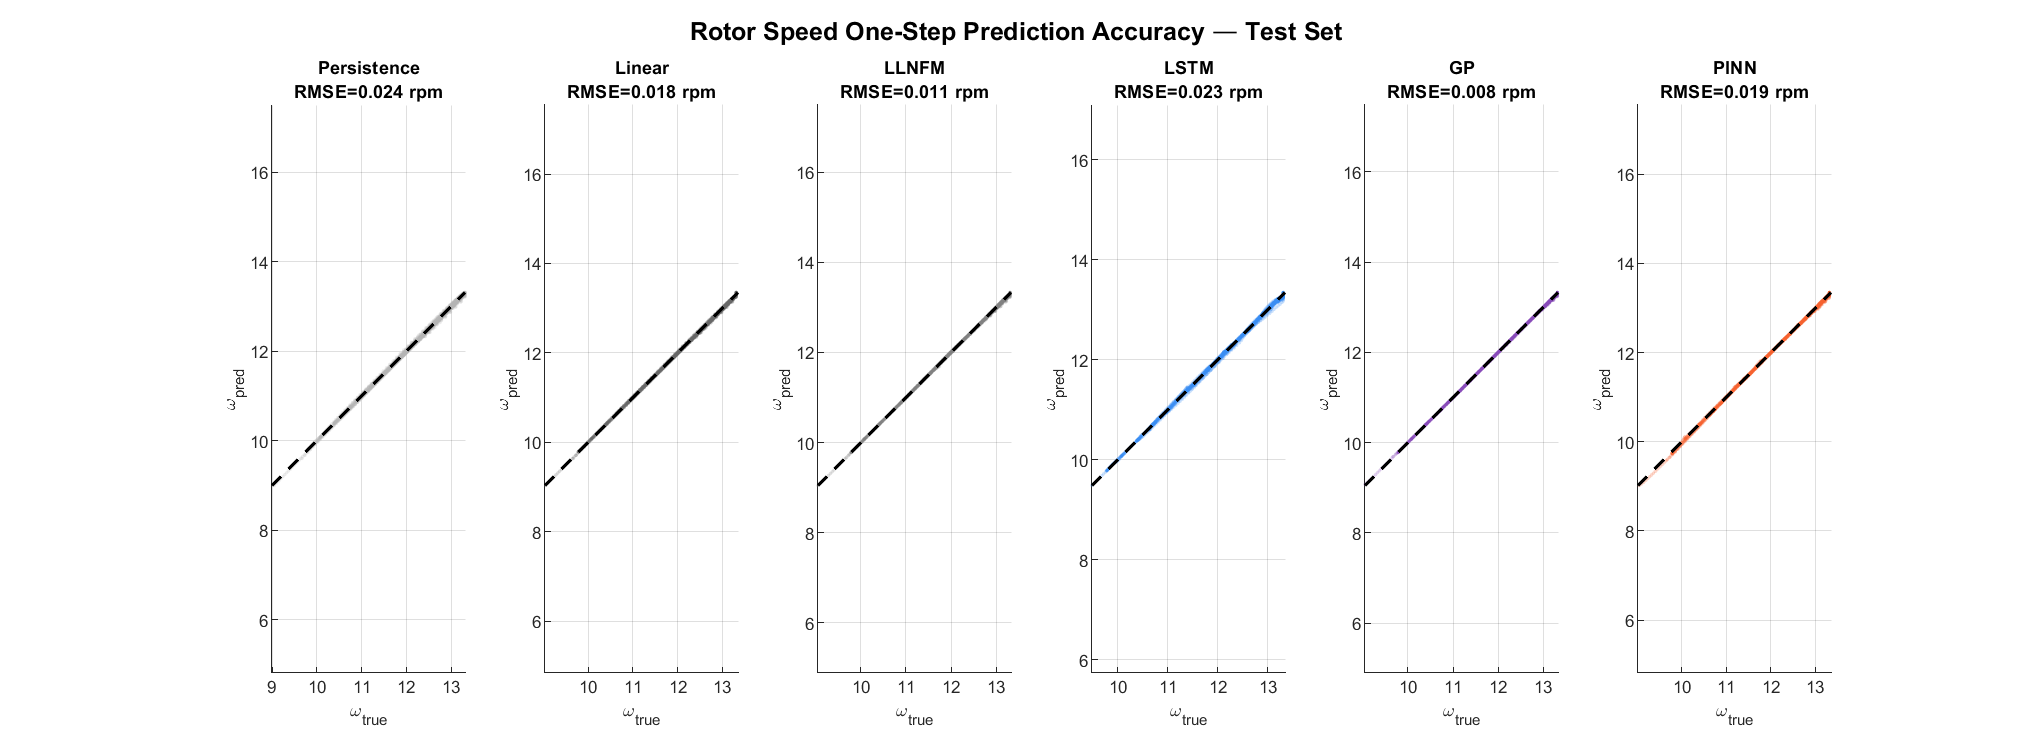
\includegraphics[width=0.85\textwidth]{figures/Fig2_S2_PredictionAccuracy.png}
\caption{Comparative test-set RMSE across all surrogate models, V1 and V2.}
\label{fig:stage2_rmse_bar}
\end{figure}
